\documentclass[]{article}
\usepackage{lmodern}
\usepackage{amssymb,amsmath}
\usepackage{ifxetex,ifluatex}
\usepackage{fixltx2e} % provides \textsubscript
\ifnum 0\ifxetex 1\fi\ifluatex 1\fi=0 % if pdftex
  \usepackage[T1]{fontenc}
  \usepackage[utf8]{inputenc}
\else % if luatex or xelatex
  \ifxetex
    \usepackage{mathspec}
  \else
    \usepackage{fontspec}
  \fi
  \defaultfontfeatures{Ligatures=TeX,Scale=MatchLowercase}
\fi
% use upquote if available, for straight quotes in verbatim environments
\IfFileExists{upquote.sty}{\usepackage{upquote}}{}
% use microtype if available
\IfFileExists{microtype.sty}{%
\usepackage{microtype}
\UseMicrotypeSet[protrusion]{basicmath} % disable protrusion for tt fonts
}{}
\usepackage[margin=1in]{geometry}
\usepackage{hyperref}
\hypersetup{unicode=true,
            pdftitle={Chapter 6 Exercise 2},
            pdfauthor={Allen Church},
            pdfborder={0 0 0},
            breaklinks=true}
\urlstyle{same}  % don't use monospace font for urls
\usepackage{color}
\usepackage{fancyvrb}
\newcommand{\VerbBar}{|}
\newcommand{\VERB}{\Verb[commandchars=\\\{\}]}
\DefineVerbatimEnvironment{Highlighting}{Verbatim}{commandchars=\\\{\}}
% Add ',fontsize=\small' for more characters per line
\usepackage{framed}
\definecolor{shadecolor}{RGB}{248,248,248}
\newenvironment{Shaded}{\begin{snugshade}}{\end{snugshade}}
\newcommand{\KeywordTok}[1]{\textcolor[rgb]{0.13,0.29,0.53}{\textbf{#1}}}
\newcommand{\DataTypeTok}[1]{\textcolor[rgb]{0.13,0.29,0.53}{#1}}
\newcommand{\DecValTok}[1]{\textcolor[rgb]{0.00,0.00,0.81}{#1}}
\newcommand{\BaseNTok}[1]{\textcolor[rgb]{0.00,0.00,0.81}{#1}}
\newcommand{\FloatTok}[1]{\textcolor[rgb]{0.00,0.00,0.81}{#1}}
\newcommand{\ConstantTok}[1]{\textcolor[rgb]{0.00,0.00,0.00}{#1}}
\newcommand{\CharTok}[1]{\textcolor[rgb]{0.31,0.60,0.02}{#1}}
\newcommand{\SpecialCharTok}[1]{\textcolor[rgb]{0.00,0.00,0.00}{#1}}
\newcommand{\StringTok}[1]{\textcolor[rgb]{0.31,0.60,0.02}{#1}}
\newcommand{\VerbatimStringTok}[1]{\textcolor[rgb]{0.31,0.60,0.02}{#1}}
\newcommand{\SpecialStringTok}[1]{\textcolor[rgb]{0.31,0.60,0.02}{#1}}
\newcommand{\ImportTok}[1]{#1}
\newcommand{\CommentTok}[1]{\textcolor[rgb]{0.56,0.35,0.01}{\textit{#1}}}
\newcommand{\DocumentationTok}[1]{\textcolor[rgb]{0.56,0.35,0.01}{\textbf{\textit{#1}}}}
\newcommand{\AnnotationTok}[1]{\textcolor[rgb]{0.56,0.35,0.01}{\textbf{\textit{#1}}}}
\newcommand{\CommentVarTok}[1]{\textcolor[rgb]{0.56,0.35,0.01}{\textbf{\textit{#1}}}}
\newcommand{\OtherTok}[1]{\textcolor[rgb]{0.56,0.35,0.01}{#1}}
\newcommand{\FunctionTok}[1]{\textcolor[rgb]{0.00,0.00,0.00}{#1}}
\newcommand{\VariableTok}[1]{\textcolor[rgb]{0.00,0.00,0.00}{#1}}
\newcommand{\ControlFlowTok}[1]{\textcolor[rgb]{0.13,0.29,0.53}{\textbf{#1}}}
\newcommand{\OperatorTok}[1]{\textcolor[rgb]{0.81,0.36,0.00}{\textbf{#1}}}
\newcommand{\BuiltInTok}[1]{#1}
\newcommand{\ExtensionTok}[1]{#1}
\newcommand{\PreprocessorTok}[1]{\textcolor[rgb]{0.56,0.35,0.01}{\textit{#1}}}
\newcommand{\AttributeTok}[1]{\textcolor[rgb]{0.77,0.63,0.00}{#1}}
\newcommand{\RegionMarkerTok}[1]{#1}
\newcommand{\InformationTok}[1]{\textcolor[rgb]{0.56,0.35,0.01}{\textbf{\textit{#1}}}}
\newcommand{\WarningTok}[1]{\textcolor[rgb]{0.56,0.35,0.01}{\textbf{\textit{#1}}}}
\newcommand{\AlertTok}[1]{\textcolor[rgb]{0.94,0.16,0.16}{#1}}
\newcommand{\ErrorTok}[1]{\textcolor[rgb]{0.64,0.00,0.00}{\textbf{#1}}}
\newcommand{\NormalTok}[1]{#1}
\usepackage{graphicx,grffile}
\makeatletter
\def\maxwidth{\ifdim\Gin@nat@width>\linewidth\linewidth\else\Gin@nat@width\fi}
\def\maxheight{\ifdim\Gin@nat@height>\textheight\textheight\else\Gin@nat@height\fi}
\makeatother
% Scale images if necessary, so that they will not overflow the page
% margins by default, and it is still possible to overwrite the defaults
% using explicit options in \includegraphics[width, height, ...]{}
\setkeys{Gin}{width=\maxwidth,height=\maxheight,keepaspectratio}
\IfFileExists{parskip.sty}{%
\usepackage{parskip}
}{% else
\setlength{\parindent}{0pt}
\setlength{\parskip}{6pt plus 2pt minus 1pt}
}
\setlength{\emergencystretch}{3em}  % prevent overfull lines
\providecommand{\tightlist}{%
  \setlength{\itemsep}{0pt}\setlength{\parskip}{0pt}}
\setcounter{secnumdepth}{0}
% Redefines (sub)paragraphs to behave more like sections
\ifx\paragraph\undefined\else
\let\oldparagraph\paragraph
\renewcommand{\paragraph}[1]{\oldparagraph{#1}\mbox{}}
\fi
\ifx\subparagraph\undefined\else
\let\oldsubparagraph\subparagraph
\renewcommand{\subparagraph}[1]{\oldsubparagraph{#1}\mbox{}}
\fi

%%% Use protect on footnotes to avoid problems with footnotes in titles
\let\rmarkdownfootnote\footnote%
\def\footnote{\protect\rmarkdownfootnote}

%%% Change title format to be more compact
\usepackage{titling}

% Create subtitle command for use in maketitle
\providecommand{\subtitle}[1]{
  \posttitle{
    \begin{center}\large#1\end{center}
    }
}

\setlength{\droptitle}{-2em}

  \title{Chapter 6 Exercise 2}
    \pretitle{\vspace{\droptitle}\centering\huge}
  \posttitle{\par}
    \author{Allen Church}
    \preauthor{\centering\large\emph}
  \postauthor{\par}
      \predate{\centering\large\emph}
  \postdate{\par}
    \date{11/6/2019}


\begin{document}
\maketitle

\begin{Shaded}
\begin{Highlighting}[]
\KeywordTok{require}\NormalTok{(knitr)}
\end{Highlighting}
\end{Shaded}

\begin{verbatim}
## Loading required package: knitr
\end{verbatim}

\begin{Shaded}
\begin{Highlighting}[]
\KeywordTok{require}\NormalTok{(haven)}
\end{Highlighting}
\end{Shaded}

\begin{verbatim}
## Loading required package: haven
\end{verbatim}

\begin{Shaded}
\begin{Highlighting}[]
\NormalTok{opts_chunk}\OperatorTok{$}\KeywordTok{set}\NormalTok{(}\DataTypeTok{echo =} \OtherTok{TRUE}\NormalTok{)}
\KeywordTok{options}\NormalTok{(}\DataTypeTok{digits =} \DecValTok{3}\NormalTok{)}

\KeywordTok{load}\NormalTok{(}\StringTok{"Ch6_Exercise2_FederalReserve.RData"}\NormalTok{)}

\CommentTok{#Add working directory, assign data to lab variable}
\KeywordTok{View}\NormalTok{(dta)}
\end{Highlighting}
\end{Shaded}

2a. Democrat scatterplot

\begin{Shaded}
\begin{Highlighting}[]
\CommentTok{#Subset dataset and specify Democrat column to equal 1}
\NormalTok{dem_plot <-}\StringTok{ }\KeywordTok{subset}\NormalTok{(dta, dta}\OperatorTok{$}\NormalTok{Democrat}\OperatorTok{==}\DecValTok{1}\NormalTok{)}

\KeywordTok{plot}\NormalTok{(dem_plot}\OperatorTok{$}\NormalTok{Quarters, dem_plot}\OperatorTok{$}\NormalTok{FEDFUNDS, }\DataTypeTok{main=}\StringTok{"Quarters and Federal Funds Rate: Democrats"}\NormalTok{,}
     \DataTypeTok{xlab=}\StringTok{"Quarters Since Previous Election"}\NormalTok{, }\DataTypeTok{ylab =} \StringTok{"Federal Funds Rate (%)"}\NormalTok{, }\DataTypeTok{pch =} \DecValTok{19}\NormalTok{, }\DataTypeTok{col=}\StringTok{'blue'}\NormalTok{)}
\end{Highlighting}
\end{Shaded}

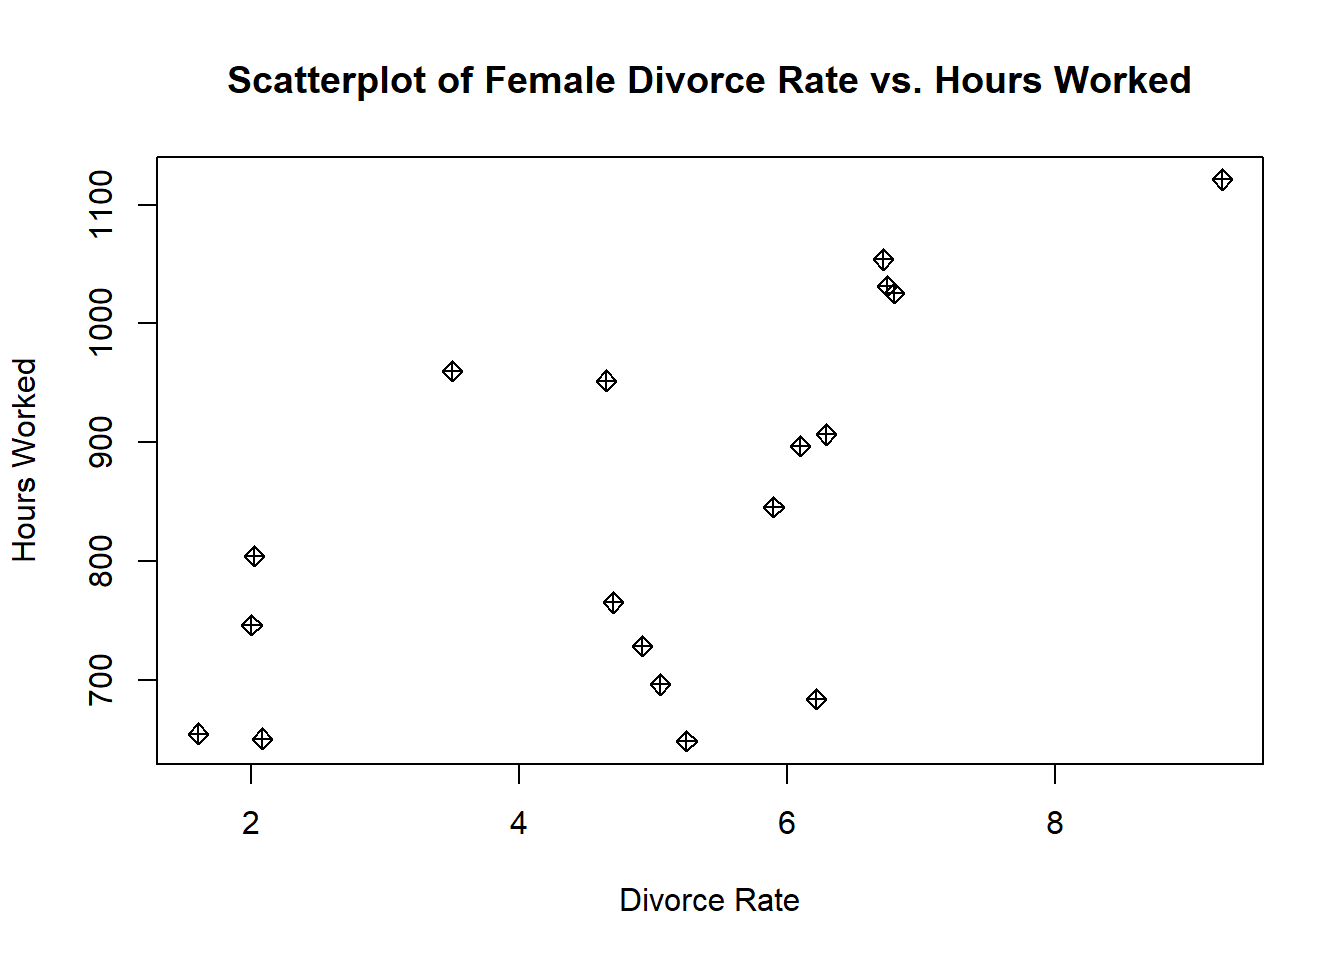
\includegraphics{ch6_ex2_files/figure-latex/unnamed-chunk-2-1.pdf}

Republican Scatterplot

\begin{Shaded}
\begin{Highlighting}[]
\CommentTok{#Subset dataset and specify Democrat column to equal 0}
\NormalTok{rep_plot <-}\StringTok{ }\KeywordTok{subset}\NormalTok{(dta, dta}\OperatorTok{$}\NormalTok{Democrat}\OperatorTok{==}\DecValTok{0}\NormalTok{)}

\KeywordTok{plot}\NormalTok{(rep_plot}\OperatorTok{$}\NormalTok{Quarters, rep_plot}\OperatorTok{$}\NormalTok{FEDFUNDS, }\DataTypeTok{main=}\StringTok{"Quarters and Federal Funds Rate: Republicans"}\NormalTok{,}
     \DataTypeTok{xlab=}\StringTok{"Quarters Since Previous Election"}\NormalTok{, }\DataTypeTok{ylab =} \StringTok{"Federal Funds Rate (%)"}\NormalTok{, }\DataTypeTok{pch =} \DecValTok{19}\NormalTok{, }\DataTypeTok{col =} \StringTok{"red"}\NormalTok{)}
\end{Highlighting}
\end{Shaded}

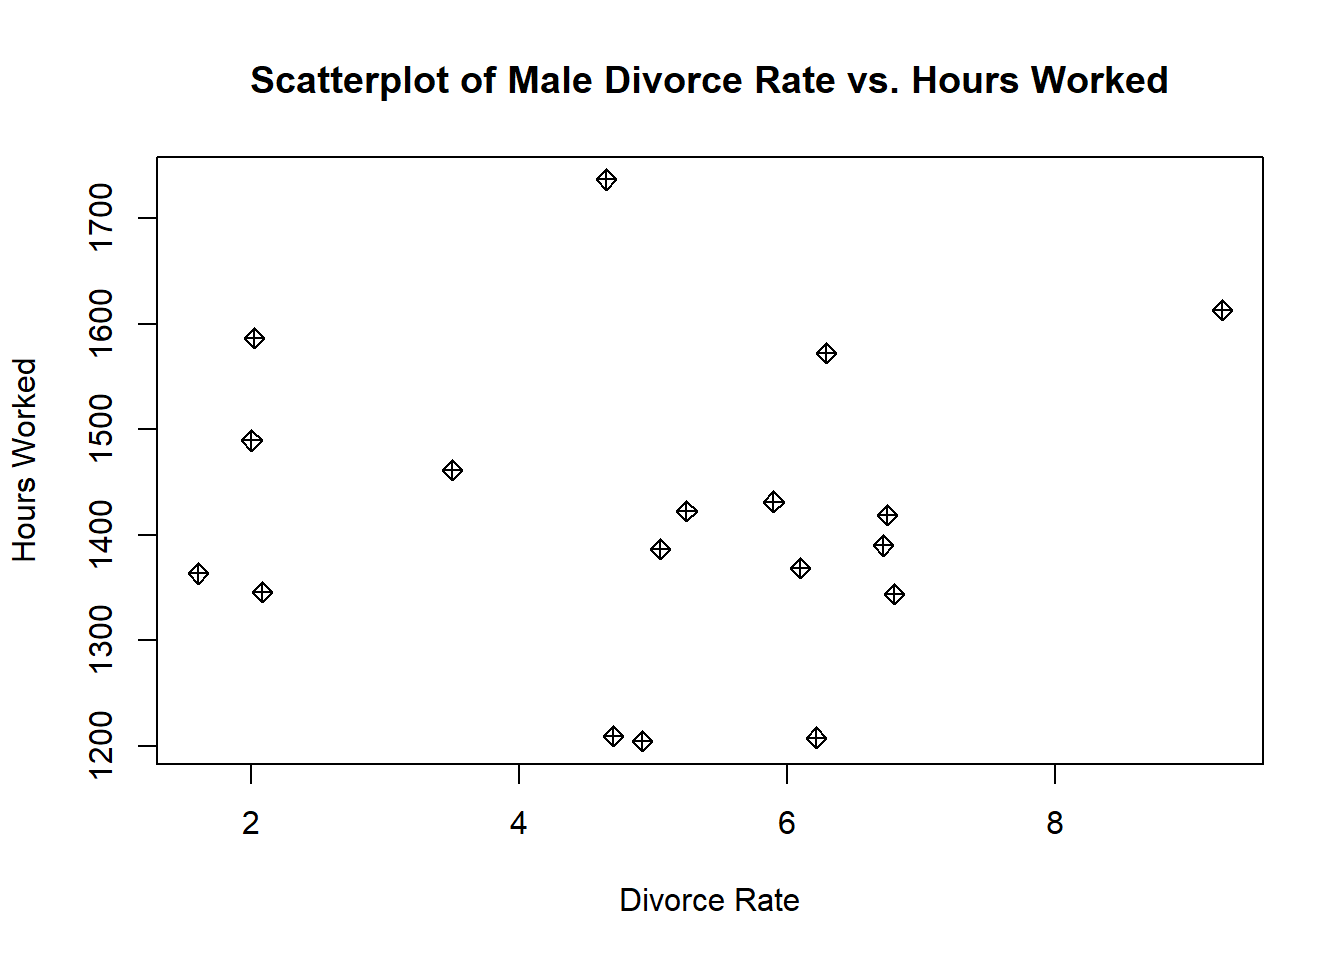
\includegraphics{ch6_ex2_files/figure-latex/unnamed-chunk-3-1.pdf}

2b. Create interaction variable between Quarters and Democrat to test
whether closeness to Quarters has the same effect on Democrats and
Republicans. Run model with FFR as dependent variable, allowing effect
of Quarters variable to vary by party of president.

\begin{Shaded}
\begin{Highlighting}[]
\CommentTok{#Create interaction variable by multiplying Democrat dummy variable with Quarters}
\NormalTok{dta}\OperatorTok{$}\NormalTok{duminteract <-}\StringTok{ }\NormalTok{dta}\OperatorTok{$}\NormalTok{Democrat }\OperatorTok{*}\StringTok{ }\NormalTok{dta}\OperatorTok{$}\NormalTok{Quarters}

\CommentTok{#Run model with FFR as dependent variable and Democrat, Quarters, and duminteract as independent variables}
\NormalTok{olsinteraction <-}\StringTok{ }\KeywordTok{lm}\NormalTok{(dta}\OperatorTok{$}\NormalTok{FEDFUNDS }\OperatorTok{~}\StringTok{ }\NormalTok{dta}\OperatorTok{$}\NormalTok{Democrat }\OperatorTok{+}\StringTok{ }\NormalTok{dta}\OperatorTok{$}\NormalTok{Quarters }\OperatorTok{+}\StringTok{ }\NormalTok{dta}\OperatorTok{$}\NormalTok{duminteract)}
\KeywordTok{summary}\NormalTok{(olsinteraction)}
\end{Highlighting}
\end{Shaded}

\begin{verbatim}
## 
## Call:
## lm(formula = dta$FEDFUNDS ~ dta$Democrat + dta$Quarters + dta$duminteract)
## 
## Residuals:
##    Min     1Q Median     3Q    Max 
## -5.506 -1.997 -0.365  1.661 10.339 
## 
## Coefficients:
##                 Estimate Std. Error t value Pr(>|t|)    
## (Intercept)       7.7703     0.5274   14.73  < 2e-16 ***
## dta$Democrat     -4.9032     0.8153   -6.01  7.4e-09 ***
## dta$Quarters     -0.2649     0.0588   -4.51  1.1e-05 ***
## dta$duminteract   0.5582     0.0939    5.94  1.1e-08 ***
## ---
## Signif. codes:  0 '***' 0.001 '**' 0.01 '*' 0.05 '.' 0.1 ' ' 1
## 
## Residual standard error: 3.16 on 222 degrees of freedom
##   (6 observations deleted due to missingness)
## Multiple R-squared:  0.151,  Adjusted R-squared:  0.14 
## F-statistic: 13.2 on 3 and 222 DF,  p-value: 6.08e-08
\end{verbatim}

2b. i. What change in FFR is associated with a 1 unit increase in
Quarters variable when president is republican? There is a -0.2649
change in FFR associated with a 1 unit increase in the Quarters variable
when the president is Republican.

2b. ii. What change in FFR is associated with a 1 unit increase in
Quarters variable when president is Democrat? There is a 0.5582 change
in FFR associated with a 1 unit increase in the Quarters variable when
the president is Democrat.

2c. Is the effect of Quarters statistically significant under
Republicans?

\begin{Shaded}
\begin{Highlighting}[]
\NormalTok{olsrepublican <-}\StringTok{ }\KeywordTok{lm}\NormalTok{(rep_plot}\OperatorTok{$}\NormalTok{FEDFUNDS }\OperatorTok{~}\StringTok{ }\NormalTok{rep_plot}\OperatorTok{$}\NormalTok{Quarters)}
\KeywordTok{summary}\NormalTok{(olsrepublican)}
\end{Highlighting}
\end{Shaded}

\begin{verbatim}
## 
## Call:
## lm(formula = rep_plot$FEDFUNDS ~ rep_plot$Quarters)
## 
## Residuals:
##    Min     1Q Median     3Q    Max 
## -5.506 -2.293 -0.044  1.734 10.339 
## 
## Coefficients:
##                   Estimate Std. Error t value Pr(>|t|)    
## (Intercept)          7.770      0.566    13.7  < 2e-16 ***
## rep_plot$Quarters   -0.265      0.063    -4.2  4.8e-05 ***
## ---
## Signif. codes:  0 '***' 0.001 '**' 0.01 '*' 0.05 '.' 0.1 ' ' 1
## 
## Residual standard error: 3.39 on 136 degrees of freedom
##   (6 observations deleted due to missingness)
## Multiple R-squared:  0.115,  Adjusted R-squared:  0.108 
## F-statistic: 17.7 on 1 and 136 DF,  p-value: 4.77e-05
\end{verbatim}

The coefficient on Quarters under Republicans is negative (-0.265) with
a t statistic of 4.2, implying it is statistically significant.

Is the effect of Quarters statistically significant under Democrats?

\begin{Shaded}
\begin{Highlighting}[]
\NormalTok{olsDemocrat <-}\StringTok{ }\KeywordTok{lm}\NormalTok{(dem_plot}\OperatorTok{$}\NormalTok{FEDFUNDS }\OperatorTok{~}\StringTok{ }\NormalTok{dem_plot}\OperatorTok{$}\NormalTok{Quarters)}
\KeywordTok{summary}\NormalTok{(olsDemocrat)}
\end{Highlighting}
\end{Shaded}

\begin{verbatim}
## 
## Call:
## lm(formula = dem_plot$FEDFUNDS ~ dem_plot$Quarters)
## 
## Residuals:
##    Min     1Q Median     3Q    Max 
## -4.730 -1.736 -0.432  1.119  8.663 
## 
## Coefficients:
##                   Estimate Std. Error t value Pr(>|t|)    
## (Intercept)          2.867      0.543    5.28  9.7e-07 ***
## dem_plot$Quarters    0.293      0.064    4.58  1.5e-05 ***
## ---
## Signif. codes:  0 '***' 0.001 '**' 0.01 '*' 0.05 '.' 0.1 ' ' 1
## 
## Residual standard error: 2.76 on 86 degrees of freedom
## Multiple R-squared:  0.196,  Adjusted R-squared:  0.187 
## F-statistic:   21 on 1 and 86 DF,  p-value: 1.54e-05
\end{verbatim}

The coefficient on Quarters under Democrats is positive (0.293) with a t
statistic of 4.58, implying it is statistically significant.

2d. Fitted lines for relationship between Quarters and interest rates

\begin{Shaded}
\begin{Highlighting}[]
\CommentTok{#View(dta)}
\KeywordTok{plot}\NormalTok{(dem_plot}\OperatorTok{$}\NormalTok{Quarters, dem_plot}\OperatorTok{$}\NormalTok{FEDFUNDS, }\DataTypeTok{main=}\StringTok{"Quarters and Federal Funds Rate"}\NormalTok{,}
     \DataTypeTok{xlab=}\StringTok{"Quarters Since Previous Election"}\NormalTok{, }\DataTypeTok{ylab =} \StringTok{"Federal Funds Rate (%)"}\NormalTok{, }\DataTypeTok{pch=}\DecValTok{19}\NormalTok{, }\DataTypeTok{col=}\StringTok{'blue'}\NormalTok{)}
\KeywordTok{points}\NormalTok{(rep_plot}\OperatorTok{$}\NormalTok{Quarters, rep_plot}\OperatorTok{$}\NormalTok{FEDFUNDS, }\DataTypeTok{pch=}\DecValTok{18}\NormalTok{, }\DataTypeTok{col=}\StringTok{'red'}\NormalTok{)}
\KeywordTok{abline}\NormalTok{(}\KeywordTok{lm}\NormalTok{(dem_plot}\OperatorTok{$}\NormalTok{FEDFUNDS }\OperatorTok{~}\StringTok{ }\NormalTok{dem_plot}\OperatorTok{$}\NormalTok{Quarters), }\DataTypeTok{col =} \StringTok{'blue'}\NormalTok{)}
\KeywordTok{abline}\NormalTok{(}\KeywordTok{lm}\NormalTok{(rep_plot}\OperatorTok{$}\NormalTok{FEDFUNDS }\OperatorTok{~}\StringTok{ }\NormalTok{rep_plot}\OperatorTok{$}\NormalTok{Quarters), }\DataTypeTok{col =} \StringTok{'red'}\NormalTok{)}
\KeywordTok{legend}\NormalTok{(}\StringTok{"topleft"}\NormalTok{, }\DataTypeTok{legend =} \KeywordTok{c}\NormalTok{(}\StringTok{"Democrat"}\NormalTok{, }\StringTok{"Republican"}\NormalTok{), }\DataTypeTok{pch=}\KeywordTok{c}\NormalTok{(}\DecValTok{19}\NormalTok{, }\DecValTok{18}\NormalTok{), }\DataTypeTok{col=}\KeywordTok{c}\NormalTok{(}\StringTok{"blue"}\NormalTok{, }\StringTok{"red"}\NormalTok{))}
\end{Highlighting}
\end{Shaded}

\includegraphics{ch6_ex2_files/figure-latex/unnamed-chunk-7-1.pdf} The
fitted lines above imply that for Democratic presidents, the Federal
Funds Rate gradually increases as Quarters since previous election
increase. Conversely, the fitted line for Republican presidents implies
that the Federal Funds Rate gradually decreases as Quarters since
previous election increase. These differing trends in Federal Funds
Rates imply that the Federal Reserve is not entirely free from political
influence.

2e.

\begin{Shaded}
\begin{Highlighting}[]
\NormalTok{olsinteraction_lag <-}\StringTok{ }\KeywordTok{lm}\NormalTok{(dta}\OperatorTok{$}\NormalTok{FEDFUNDS }\OperatorTok{~}\StringTok{ }\NormalTok{dta}\OperatorTok{$}\NormalTok{Democrat }\OperatorTok{+}\StringTok{ }\NormalTok{dta}\OperatorTok{$}\NormalTok{Quarters }\OperatorTok{+}\StringTok{ }\NormalTok{dta}\OperatorTok{$}\NormalTok{duminteract }\OperatorTok{+}\StringTok{ }\NormalTok{dta}\OperatorTok{$}\NormalTok{lag_FEDFUNDS }\OperatorTok{+}\StringTok{ }\NormalTok{dta}\OperatorTok{$}\NormalTok{inflation)}
\KeywordTok{summary}\NormalTok{(olsinteraction_lag)}
\end{Highlighting}
\end{Shaded}

\begin{verbatim}
## 
## Call:
## lm(formula = dta$FEDFUNDS ~ dta$Democrat + dta$Quarters + dta$duminteract + 
##     dta$lag_FEDFUNDS + dta$inflation)
## 
## Residuals:
##    Min     1Q Median     3Q    Max 
## -3.073 -0.362  0.020  0.403  5.299 
## 
## Coefficients:
##                  Estimate Std. Error t value Pr(>|t|)    
## (Intercept)        0.2463     0.2056    1.20     0.23    
## dta$Democrat      -0.1117     0.2425   -0.46     0.65    
## dta$Quarters      -0.0230     0.0168   -1.37     0.17    
## dta$duminteract    0.0470     0.0276    1.70     0.09 .  
## dta$lag_FEDFUNDS   0.8893     0.0237   37.54  < 2e-16 ***
## dta$inflation      0.1165     0.0247    4.72  4.2e-06 ***
## ---
## Signif. codes:  0 '***' 0.001 '**' 0.01 '*' 0.05 '.' 0.1 ' ' 1
## 
## Residual standard error: 0.865 on 219 degrees of freedom
##   (7 observations deleted due to missingness)
## Multiple R-squared:  0.937,  Adjusted R-squared:  0.935 
## F-statistic:  648 on 5 and 219 DF,  p-value: <2e-16
\end{verbatim}

After incorporating lag\_FEDFUNDS and inflation into the model above,
the statistical significance of the previously included coefficients
drops below 2. Specifically, the Democrat, Quarters, and duminteract
coefficients change their t statistics to 0.46, 1.37, and 1.7,
respectively. However, including the lag\_FEDFUNDS coefficient indicates
this is highly statistically significant, with a t statistic of 37.54.
Interestingly, including inflation produces a t statistic of only 4.72,
which while statistically significant, is not as significant as the
lag\_FEDFUNDS coefficient. Running the model with these included
variables indicates that lagged effective federal funds rate and
inflation rate have statistically significant - yet differing - effects
on effective federal funds rate.


\end{document}
